\documentclass{beamer}

% packages
\usepackage{graphicx,amsmath,amsfonts,amssymb,listings,tikz}

% themes & colors
\usetheme{Montpellier}
%\usecolortheme{beaver}
%\beamerdefaultoverlayspecification{<+->}

% user commands
\newcommand{\weeknum}{0}

\begin{document}

  \section{Group Meeting}
  \title{Group Meeting \\ Week \weeknum, Fall 2019}
  \author{Brandon Gusto}

  \institute{Dept. of Scientific Computing \\ Florida State University}
  \date{\today}
  \frame{\titlepage}

  \begin{frame}{Task List (DONE)}
    \begin{block}{Tasks}
      \begin{itemize}
        \setlength\itemsep{1em}
        \item Overloaded functions for multi-dimensions: \texttt{cmap} (total block mapping), \texttt{imap} (interior block mapping)
        \item Accessing neighboring leaf blocks: \texttt{gr\_findAllNeghID}
        \item Almost done building mask in 2D (8 cases: 4 face neighb's $+$ 4 corner neighb's)
        \item For periodic conditions, does function automatically give me block on other side of domain if at an edge?
      \end{itemize}
    \end{block}
  \end{frame}

  \begin{frame}{\texttt{gr\_findAllNeghID}}
    \begin{block}{Function usage}
      \texttt{neighBlkID = surrBlksSummary \% regionInfo(LEFT\_EDGE,LEFT\_EDGE,1) \& \% details(BLKNO,1)}
    \end{block}
  \end{frame}

  \begin{frame}{Implementation of Multiresolution Scheme in Proteus}
    \begin{figure}
      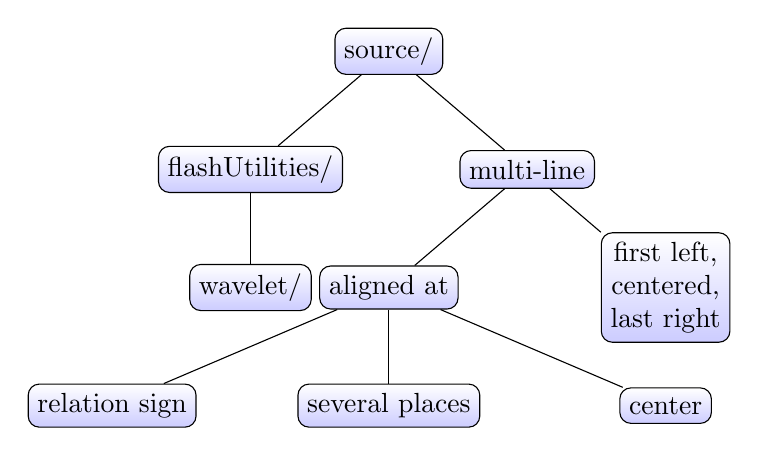
\begin{tikzpicture}[sibling distance=10em,
  every node/.style = {shape=rectangle, rounded corners,
    draw, align=center,
    top color=white, bottom color=blue!20}]
  \node {source/}
    child { node {flashUtilities/}
      child { node {wavelet/} } }
    child { node {multi-line}
      child { node {aligned at}
        child { node {relation sign} }
        child { node {several places} }
        child { node {center} } }
      child { node {first left,\\centered,\\last right} } };
\end{tikzpicture}

    \end{figure}
  \end{frame}

  \begin{frame}{Task List (TO-BE-COMPLETED)}
    \begin{block}{Tasks}
      \begin{itemize}
        \setlength\itemsep{1em}
        \item Parallel communication of mask information to blocks across processors (in 1D and 2D)
        \item Last thing in 2D is to implement interpolation in \texttt{prolong\_gen\_unk1\_fun}
        \item Prolongation gets called both for whole block refinement and for coarse-to-fine ghost cell operations
        \item Restriction is left as-is in all dimensions
      \end{itemize}
    \end{block}
  \end{frame}

\end{document}
